\subsection{Zadanie 9}

Gęstość zmiennej losowej $X$ o rozkładzie wykładniczym z parametrem $\lambda$ jest dana przez 
$$
f(x) = \left\{
\begin{array}{lcr}
\lambda \cdot e^{-\lambda x} & \text{gdy} & x > 0\\
0 & \text{gdy} & x \leq 0
\end{array}
\right.
$$

Zatem jeżeli za parametr  $\lambda$  przyjmiemy 1 otrzymamy:

$$
f(x) = \left\{
\begin{array}{rcl}
e^{- x} & \text{gdy} & x > 0\\
0 & \text{gdy} & x \leq 0
\end{array}
\right.
$$
  
Co przedstawione zostało na rysunku.

\begin{center}
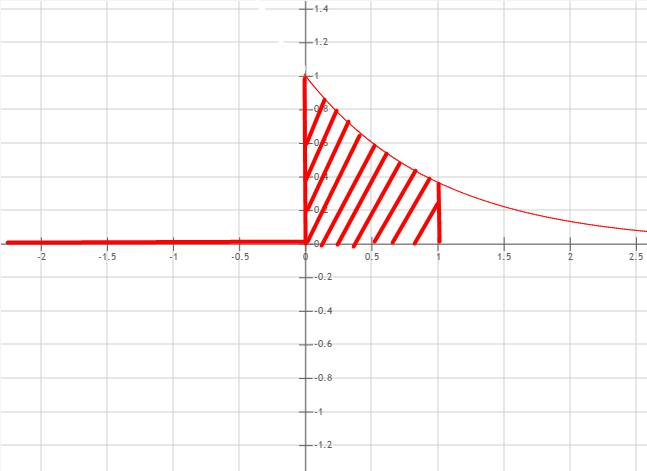
\includegraphics[width=12cm]{./tydzien_04/zad_09.png}
\end{center}

Prawdopodobieństwo, że  $X \in [0,1]$ zostało przedstawione na rysunku poprzez obszar zakreskowany na czerwono.

Obliczmy prawdopodobieństwo zdarzenia że $X \in [0,1]$:

$$
\int_{0}^{1} e^{- x} dx = [-e^x]_{0}^{1} = -e^{-1} + 1
$$
